\section{Versuchsdurchführung}
\label{sec:durchfuerung}

Der Versuch wurde mit dem Einschalten des Thermostaten zur Temperaturegelung des Temperiermantels um das Probengefäßes begonnen. Der \textsc{Du-Noüy}-Ring wurde, wie auch das Probengefäß, in Aceton gespült und in den dafür vorgesehenen Haken am Waagebalken eingehängt. Die Plattform des Tensiometers wurde anhand der eingebauten Libelle auf einen geraden Stand überprüft.  Die Nachfolgende Prozedur wiederholt sich bei jeder Messung. 
Der Probentisch wurde bis zur Markierung nach oben ausgefahren und so eingestellt, dass der sich der Ring am Waagebalken in Nullstellung  etwa \SI{5}{\milli\meter} unterhalb des Flüssigkeitspiegels befindet. Gegebenenfalls muss er leicht mit dem Finger nach unten gedrückt werden, da er beim Eintauchen an der Oberfläche haften bleibt. Die Nachfolgende Prozedur wiederholt sich bei jeder Messung. Während der Messungen sind drei Handlungen gleichzeitig auszuführen. Der Probentisch wird behutsam durch Betätigung des Stellrades nach unten gefahren. Dabei wird überwacht, ob der Waagebalken sich aus ddem Weißen bereich der Markierung bewegt. Der eintretenden Bewegung nach unten wird, durch Drehen am Handrad mit dem Zeiger über der Skala, entgegengewirkt. sobald der Flüssigkeitsfilm am Ring abreißt sind alle Drehbewegungen sofort einzustellen. Nun kann die Aufgebrachte Kraft auf der Skala abgelesen werden.

Auf oben genannte Weise wird zuerst die Kalibrierung durchgeführt. Dabei wird die Oberflächenspannung von bidestilliertem Wasser, bei \SI{20}{\degreeCelsius} mit dem Erwartungswert von \SI{72,8}{\milli\newton\per\meter} verglichen. Daraus ergibt sich, der für spätere Rechnungen bedeutsame Apparatekorrekturfaktor K$_{\text{Ka}}$.

Nach der Kalibrierung sind die wässrigen Lösungen von fit-Geschirrspülmittel, Natriumdodecylsulfat, Ethanol und Natriumchlorid bei \SI{20}{\degreeCelsius} auf ihre Oberflächenspannung zu untersuchen. Dabei werden in \SI{100}{\milli\liter}-Maßkolben jeweils 0,1 molare Lösungen von Natriumchlorid und Ethanol hergestellt. Das Natriumdodecylsulfat wird auf eine Konzentration von \SI{0,001}{\mole\per\liter} verdünnt. Beim fit reicht es einen Tropfen im Probengefäß mit destilliertem Wasser aufzufüllen. Die berechneten und verwendeten Massen und Volumina zur Herstellung der Lösungen sind auf dem Vordruck und Deckblatt zur Versuchsdurchführung eingetragen. 

Schließlich wird noch die Entwicklung der Oberflächenspannung des Bidestillierten Wassers bei Temperaturen zwischen \SI{20}{\degreeCelsius} und\SI{60}{\degreeCelsius} durch Fünfach-messung der Oberflächenspannung bei \SI{30}{\degreeCelsius}, \SI{40}{\degreeCelsius} und \SI{60}{\degreeCelsius} untersucht. Dabei können die zur Kalibrierung für die Temperatur von \SI{20}{\degreeCelsius} aufgenommenen Daten noch einmal verwendet werden. Aus Zeitgründen wurden für die Temperaturen von \SI{40}{\degreeCelsius} und \SI{60}{\degreeCelsius} gegebene Werte eines früheren Experiments übernommen.

Das Ablesen an der Skala konnte nicht mit Nachkommastellen erfolgen. Selbige wurden aufgrund der Zeigerstellungen zwischen den Markierungen abgeschätzt.




\begin{figure}[h!]
\centering
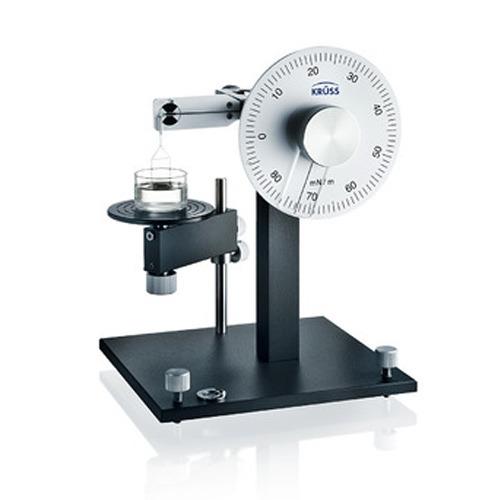
\includegraphics[width=0.7\linewidth]{img/tensiometer}
\caption{Das verwendete Tensiometer}
\label{fig:versuchsaufbau-ebull}
\end{figure}

